\documentclass{article}

% If you're new to LaTeX, here's some short tutorials:
% https://www.overleaf.com/learn/latex/Learn_LaTeX_in_30_minutes
% https://en.wikibooks.org/wiki/LaTeX/Basics

% Formatting
\usepackage[utf8]{inputenc}
\usepackage[margin=1in]{geometry}
\usepackage[titletoc,title]{appendix}

% Math
% https://www.overleaf.com/learn/latex/Mathematical_expressions
% https://en.wikibooks.org/wiki/LaTeX/Mathematics
\usepackage{amsmath,amsfonts,amssymb,amsthm,mathtools}

% Images
% https://www.overleaf.com/learn/latex/Inserting_Images
% https://en.wikibooks.org/wiki/LaTeX/Floats,_Figures_and_Captions
\usepackage{graphicx,float}
\usepackage{tikz, tikz-3dplot}

% Tables
% https://www.overleaf.com/learn/latex/Tables
% https://en.wikibooks.org/wiki/LaTeX/Tables

% Algorithms
% https://www.overleaf.com/learn/latex/algorithms
% https://en.wikibooks.org/wiki/LaTeX/Algorithms
\usepackage[ruled,vlined]{algorithm2e}
\usepackage{algorithmic}

% Code syntax highlighting
% https://www.overleaf.com/learn/latex/Code_Highlighting_with_minted
\usepackage{minted}
\usemintedstyle{borland}

% References
% https://www.overleaf.com/learn/latex/Bibliography_management_in_LaTeX
% https://en.wikibooks.org/wiki/LaTeX/Bibliography_Management
\usepackage[sorting=none]{biblatex}
\addbibresource{references.bib}

\usepackage{tikz}
\usepackage{tkz-euclide}
\usetikzlibrary{arrows.meta}
\usetikzlibrary{decorations.markings}
\usetikzlibrary{decorations.pathmorphing}
\usetikzlibrary{positioning}
\usetikzlibrary{fadings}
\usetikzlibrary{intersections}
\usetikzlibrary{cd}
\newcommand*\circled[1]{\tikz[baseline=(char.base)]{
            \node[shape=circle,draw,inner sep=2pt] (char) {#1};}}
\pgfarrowsdeclarecombine{twolatex'}{twolatex'}{latex'}{latex'}{latex'}{latex'}
\tikzset{->/.style = {decoration={markings,
                                  mark=at position 1 with {\arrow[scale=2]{latex'}}},
                      postaction={decorate}}}
\tikzset{->-/.style = {decoration={markings,
                                   mark=at position #1 with {\arrow[scale=2]{latex'}}},
                       postaction={decorate}}}
\usepackage{braket}
\usetikzlibrary{backgrounds,quantikz,shapes}

\theoremstyle{definition}
\newtheorem*{eg}{Example}
\newtheorem{lem}{Lemma}[section]
\newtheorem{cor}{Corollary}[section]
\newtheorem{thm}{Theorem}[section]
\newtheorem{defi}{Definition}[section]
\newtheorem*{remark}{Remark}
\newtheorem*{notation}{Notation}

\usepackage{tikz}
\usetikzlibrary{backgrounds,quantikz,shapes}

\def\contra{\tikz[baseline, x=0.22em, y=0.22em, line width=0.032em]\draw (0,2.83)--(2.83,0) (0.71,3.54)--(3.54,0.71) (0,0.71)--(2.83,3.54) (0.71,0)--(3.54,2.83);} 

\usepackage{fancyhdr}
\pagestyle{fancy}
\usepackage[ color={[gray]{0.8}},
 text=DRAFT\\COPY]{draftwatermark}
\fancyhf{}

\lhead{\rightmark}
\chead{DRAFT}
\cfoot{\thepage}

\renewcommand{\headrulewidth}{2pt}
\renewcommand{\footrulewidth}{1pt}


\newcommand{\HRule}[1]{\rule{\linewidth}{#1}} 	% Horizontal rule

\makeatletter							% Title
\def\printtitle{%						
    {\centering \@title\par}}
\makeatother									

\makeatletter							% Author
\def\printauthor{%					
    {\centering \large \@author}}				
\makeatother	


\title{
			\HRule{0.5pt} \\						% Upper rule
			\LARGE \textbf{\uppercase{Quantum Machine Learning: State-of-the-Art Report and How-to Guide (Provisional Title)}}	% Title
			\HRule{2pt} \\ [0.5cm]		% Lower rule + 0.5cm spacing
			\normalsize \today			% Todays date
		}




\author{Joseph Tedds - joseph.tedds@astrazeneca.com \\
 Domingo Salazar - domingo.salazar@astrazeneca.com}

%\date{29/07/20}

\begin{document}
\maketitle
\clearpage



\section{Executive Summary}
The 21st century has brought us into a quantum revolution, much like the digital revolution and the recent machine learning influx, we hope to be able to utilise these to aid our work.

\begin{itemize}
\item \textbf{Quantum Computing} - algorithms for quantum computing are theoretically able to provide exponential speed-up for certain problems. We see current uses for example in optimisation, machine learning and drug discovery, but may have further undiscovered uses.
\item \textbf{Quantum Sensing and Metrology} - In developing quantum technology, we gain side benefits from the technology in our ability to accurately measure small phenomena. We can use these for more accurate atomic clocks, the detection of magnetic field vectors, optical phase measurement and quantum state discrimination. 
\item \textbf{Quantum Internet} - One of the end goals for quantum computing is to complement the classical internet with the quantum internet. It should be able to provide secure communication, secure identification, position verification, secured dedicated computing with security based on the laws of physics rather than 'hard' mathematical problems.
\end{itemize}

What recent advances makes us think that quantum computing could be useful to AstraZeneca? 
\begin{itemize}
    \item \textbf{Shor's Algorithm} \cite{Shor_1997} appearing in 1994 was arguably the beginning of quantum hype. This provides an exponential speed-up in factoring large numbers and computing discrete logarithms. Both of these problems are important in cryptography as they provide security for a number of protocols still in use today, e.g. RSA.
    \item Preskill \cite{preskill2012quantum} defines \textbf{quantum supremacy} to be '\textit{when we will be able to perform tasks with controlled quantum systems going beyond what can be achieved with ordinary digital computers.}' In 2019, Google claimed to have achieved this \cite{quantum_supremacy}, which was shortly refuted by IBM \cite{ibm_refute} in a blog post maintaining that the calculation could be performed in $2 \frac{1}{2}$ days on a classical supercomputer. Whatever your opinion on the authenticity of this claim, this was definitely a landmark moment.
    \item With many high profile companies now competing in the hardware space: Google, IBM, Rigetti, large breakthroughs are being made in the numbers of qubits available and error rates. With a wide variety of approaches, companies expect to break the \textbf{threshold of 1000 qubits} some time in the next four years. 
    \item An increasing number of companies are also providing access to quantum computers \textbf{via the cloud}. AstraZeneca already has access Microsoft Azure Quantum, but Amazon, IBM, Google, D-Wave and Oxford Quantum Circuits all have offerings.
    \item Very recent research by IBM \cite{Liu_2021} shows a \textbf{theoretical quantum advantage} for machine learning problems given classical input. This is important since most existing quantum advantage relied on the input of quantum data, or classical data already existing in a 'nice' quantum form. 
    \item  No universal software exists for quantum computers, just many Python libraries and one new Quantum Language, Q\#. 
\end{itemize}

What challenges does quantum computing face in providing practical quantum computers and usage? A by no means exhaustive list, can be broken down into three areas, with the challenges needing to be addressed by different areas of the industry. 

\begin{itemize}
    \item Hardware: 
    \begin{itemize}
        \item Noise causing errors in qubits.
        \item Scaling quantum computers from tens of qubits to thousands of qubits.
        \item Limited numbers of operations performed per circuit.
        \item Energy costs due to cooling, close to 0K for some computers. 
    \end{itemize}
    \item Software:
    \begin{itemize}
        \item Educating programmers on available software and algorithms.
        
        \item Quantum computing theory outpaces current hardware, requiring clarity over what algorithms can be run on what devices.
    \end{itemize}
    \item Uptake:
    \begin{itemize}
        \item Costs are high, though ameliorated by cloud computing offerings.
        \item Understanding the use cases e.g. for drug discovery, optimisation and machine learning.
        \item Access to quantum computers. 
    \end{itemize}
\end{itemize}


\clearpage
\tableofcontents

\clearpage
\part{Quantum Computing: State of the Art}
In this section, we discuss the current state of quantum computing, building up some basics for comparing quantum computers and how they work. We'll also discuss the most pressing issues for implementing quantum computing, as well as potential timelines for when major milestones may occur. 


\section{The Basics of Quantum Computing}
Quantum computing is built on linear algebra, there's no way of getting around it entirely, but we'll do the best we can. If you're interested in the more rigorous treatment, we'll revisit the basics in Part II.

In classical computing, the most basic element is a bit, taking the value either 0 or 1. We can add them together, combine them into strings and use classical gates to transform bit strings. In quantum computing, we'd like to build on these ideas, but also introduce the key quantum properties of \textbf{superposition} and \textbf{entanglement}.

In quantum computing, the most basic element is a qubit, which when measured will give the value 0 or 1. It's easier to consider a classical example first. Think of spinning a coin on its edge, at this stage it doesn't have the value heads or tails, we can only talk about the probability that it lands heads or tails. Measurement, in the form of stopping the coin, collapses the superposition and allows us to read an outcome as either heads or tails. It's exactly the same with qubits. Before we measure a qubit, they can be in a \textbf{superposition} of the states 0 and 1 and measurement causes the superposition to collapse and gives an outcome of 0 or 1 (with a probability depending on the preparation of the state).

Moving onto \textbf{entanglement}, we now need to consider multiple linked coins. The simplest example is two linked coins. We spin two coins and when we measure one, the other coin becomes fixed to the same value, i.e. we always obtain either head, head or tails, tails. Entanglement is not dependent on distance, so you can create entangled qubits and separate them. In 2017, Chinese scientists successfully maintained entanglement across 1200 km \cite{Yin1140}. 

Quantum entanglement is necessary for quantum advantage, as any calculations without entanglement can be efficiently simulated by a classical computer. 

Typically, we model classical computing as a series of logic gates. In quantum computing, we have a similar circuit model that uses quantum gates, but with the caveat that they must be reversible. 


\section{What makes a good quantum computer?}
There are various different types of quantum computer, depending on how the qubits are built. We will focus only on the types of computer that are currently under development. In looking at viable quantum computers, there are a number of properties we wish to have - the DiVincenzo Criteria \cite{DiVincenzo_2000}.
\begin{itemize}
    \item \textbf{A scalable quantum system with well characterised qubits}. Good candidates for qubits are quantum 2-level systems, mimicking our coin, e.g. the up and down spin states of a spin 1/2 particle or the ground and excite states of an atom. Qubits must be able to occupy a continuum of states, and able to be entangled with one another. Well characterised also refers to its physical parameters being accurately known: the internal Hamiltonian, the presence of and coupling to other states of the qubit, the interactions with other qubits and the coupling to external fields that might be used to manipulate the state of the qubit. In the event that the system has more than 2 levels, we require that the probability of transitioning to these higher levels is very small.
    \item \textbf{The ability to initialise the state of the qubits to a simple fiducial state}. All computations have to start somewhere, typically we choose the simple state to be $\ket{0 \cdots 0}$. Furthermore, quantum error correction will require a continuous supply of qubits in a low entropy state, thus we require the ability to produce lots of these states accurately, and on demand. Note that this can be achieved by measuring states mid-algorithm and resetting them, if necessary, to the initial state.
    \item \textbf{Long relevant decoherence times, much longer than the gate operation times}. Decoherence is the process of qubits losing information due to interactions with the environment. Returning to our coin example, this is similar as letting the coin stop spinning by itself.  Amplitude damping is one such example. Say we have $\ket{0}_A$,the ground state of a 2-level atom, $\ket{1}_A$ the excited state, and $\ket{0}_E$ the environment - initially in a vacuum state. If our system is in the excited state $\ket{1}_A$, then under amplitude damping it decays to $\ket{0}_A$ with probability $p$ and spontaneous emission of a photon. In particular, we can see the decoherence of the state 
    \[
    \ket{1}_A \ket{0}_E \to \sqrt{1 - p} \ket{1}_A \ket{0}_E + \sqrt{p}\ket{0}_A\ket{1}_E.
    \]
    In general, the decoherence time will be more complex. Thus, we see in order to perform quantum calculations, we need as long a decoherence time as possible in order to obtain reliable results.
    
    \item \textbf{A ''universal" set of quantum gates}. In order to implement any general circuit, we need to be able to implement a set of gates that can generate any other gate - or a good approximation to them, i.e. with arbitrary accuracy. In classical computing, the gate set $\{\text{AND, OR, NOT} \}$ is universal. One such universal gate set for quantum computing is $\{H, CX, S, T\}$, the Hadamard, CNOT, Phase and $\pi/8$ gates. Note that the choice of universal gate set is usually determined by the choice of quantum computer, as some gates are easier to implement on one type of computer than another.
    
    \item \textbf{A qubit-specific measurement capability}. To be able to complete computations, we need to be able to read the results and know which qubits the measurements correspond to. These measurements should not cause a disturbance to any other qubits in the computer and be independent of all other physical parameters of the system. Further, we wish for these measurements to be accurate in the sense that when measuring a state with density matrix given by
    \[
    \rho = p \ket{0} \bra{0} + (1 -p) \ket{1} \bra{1} + \alpha \ket{0} \bra{1} + \alpha ^\ast \ket{1} \bra{0},
    \]
    we expect to see the result $0$ with probability $p$, and $1$ with probability $ 1-p$.
\end{itemize} 

\section{Logical and Physical Qubits}
When referring to qubits, we have been assuming that the systems are noise free. They are an ideal implementation of qubits that have long enough coherence time to be useful and are resistant to errors caused by low gate fidelity. Physical qubits are simply our actual implementation of the qubits for a given system. We can use quantum circuits to create logical qubits from our physical qubits via error correcting methods. 

Quantum error correction is a rich part of quantum information theory, and a way to protect against gate errors and decoherence. In classical computing, for example, we can use the repetition code to protect against errors:
\[
0  \to 000, \quad 1 \to 111.
\]
We can then decide the output by majority voting, i.e. if we see $010$ then we conclude the input was $0$. Quantum information has some subtleties attached to it that mean we can't simply clone states, and so a direct implementation of the repetition code is not possible. Instead, we can do things like entangling qubits with ancillary (extra) qubits. In general, far more complex error correcting schemes will be needed.

The amount of physical qubits needed to encode a logical qubit is dependent on the errors in the quantum system and the encoding system used. Sevilla and Riedel \cite{sevilla2020forecasting} define this more rigorously, with the number of \textbf{generalised logical qubits} able to be used as a comparative metric for different computers. Note that the only experimental reliance, here, is for the error rate of the two-qubit gates. 

\[
N_L = N_p f_{\text{QEC}}, \quad f_{\text{QEC}} = \left[ 4 \frac{\log (\sqrt{10} p_P/p_L)}{\log(p_{th}/p_P)} + 1 \right]^{-2}.
\]

Where:
\begin{itemize}
    \item $N_L$ is the number of logical qubits.
    \item $N_P$ is the number of physical qubits.
    \item $p_P$ is the two-qubit gate error. (We don't consider the error from gates acting on one qubit, as the two-qubit error rate is far higher).
    \item $p_{th}$ is an approximate threshold error at which fault-tolerance becomes possible (see below for more on this). 
    \item $p_L$ the two-qubit error for the logical qubits.
\end{itemize}
We are free to pick $p_L$ to be as we like, though since $1/p_L$ is on average the number of two-qubit gates we can apply before an error takes place, we want to choose this to be small enough to accomplish most algorithms. For a particular error correcting code, the surface code, Javadi-Avhari \cite{javadi-avhari_2017} gives $p_{th} \approx 10^{-2}$. Note that this formula is only an approximation. 

\begin{figure}[htb]
    \centering
    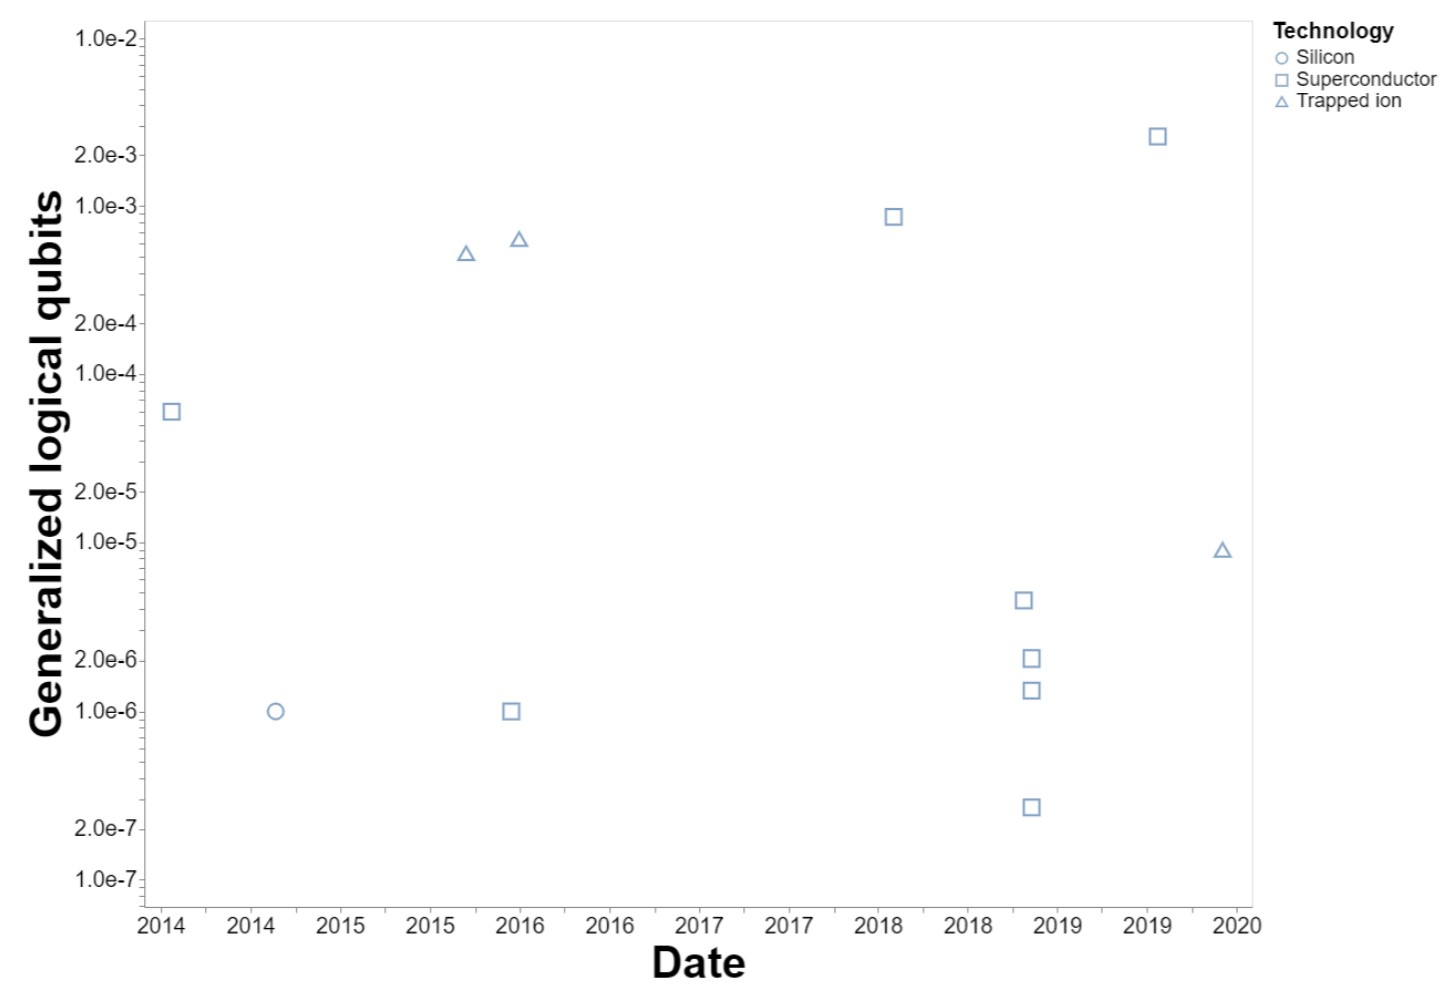
\includegraphics[scale=0.5]{generalised_qubit_amounts.jpg}
    \caption{Calculated numbers of generalised logical qubits from 2003 to 2020 (including only those meeting the fault-tolerance threshold). In: \textit{Towards a scalable software stack for resource estimation and optimization in general-purpose quantum computers} Javadi-Avhari p9. Figure 4 \cite{javadi-avhari_2017}}
    \label{fig:logical_qubit_num}
\end{figure}
As we can see in the figure above, the Rigetti Aspen-4 has the highest number of generalised logical qubits at roughly 0.003. Logical qubits are clearly our goal, as a near-perfect realisation of our algorithms. A significant milestone then is reaching one logical qubit. Perhaps a more interesting question is how many we need to run general purpose quantum algorithms. Roettler et al. \cite{roetteler2017quantum} put the number of logical qubits needed to factorise a 2048-bit number at roughly 4096 for Shor's algorithm. 

\section{Analogue, NISQ \& FTQC Computers}
Grumbling and Horowitz \cite{NAP25196} broadly define 3 different types of quantum computer. 
\begin{itemize}
    \item \textbf{Analogue Quantum Computers} - quantum computers where the dynamics of the system we use for computing is similar to the model we wish to study. We are unable to manipulate the individual steps, quantum gates, directly and can only make analogue changes to the dynamics of the quantum system. For instance, a \textbf{quantum annealer} prepares an initial state for a simple Hamiltonian and the Hamiltonian is slowly altered until it becomes the problem Hamiltonian. Since the ground state will sit in the minimum energy state, we hope to find a minimal energy solution as our final state, though there is a non-zero probability that this is an excited state. These computers are useful for sampling and optimization problems, but have problems with thermal noise and running the system too quickly can introduce errors. Note that there do exist some examples of protein folding on 2-D and 3-D lattices \cite{perdomoortiz2012finding}, \cite{babej2018coarsegrained}. 
    \item \textbf{Noisy Intermediate Scale Quantum computers (NISQ)} - these are the digital quantum computers we currently work with. These are characterised as digital, since we can manipulate the qubits via quantum gates that allow us to complete any theoretical computation. However, our current implementations are very noisy (as the name suggests) so we can't run thousands of gates without creating large errors, and we're restricted in the number of qubits we can access.
    \item \textbf{Fault Tolerant Quantum Computer (FTQC)} - Digital quantum computers using logical qubits. This is the end goal of quantum computing. Since the gate-based calculations are now error free (up to an arbitrary amount) we would be able to complete algorithms of increased complexity and depth, hence utilise the full power of quantum computing.
\end{itemize}

\section{Physical Realisations}
There are quite a few different methods to construct a quantum computer. We will very briefly discuss only a few of the more widely used types within NISQ computers.

\begin{itemize}
    \item \textbf{Superconducting quantum computers} are under development by companies like Google, IBM, Rigetti and D-Wave. The quantum system is formed by small current on a chip that quantum tunnels through a Josephson Junction. These circuits are typically 2-D, but Oxford Quantum Circuits has recently announced their 3-D circuits. The qubits are realised as charge distributions, the flux of the current, or a hybrid approach. Since these are essentially microchips, similar manufacturing techniques can be used to create them, so they are very scalable. However, the superconductivity needs the chip to be cooled to below 100 mK which is both energy and space intensive. Difficulty will also come when the system is scaled up to thousands of qubits, when multiple cooling systems may be required. While the decoherence time for the qubits is typically very fast, in the order of $10 \, \mu \text{s}$, gate application times are low enough to implement 
    \item \textbf{Trapped ion computers}. Honeywell and IonQ are the leaders in this field. The quantum system is formed by the movement of the ions suspended in electromagnetic fields, with entanglement created via lasers. Ion traps typically have longer decoherence times that superconducting qubits, and allow for greater connectivity (number of nearby qubits that can interact). However, the speed at which they operate can be quite slow and adding qubits becomes more difficult due to unwanted interactions between neighbouring ions. Furthermore, cooling is also required to below 2K, which although low requires far less energy than the superconducting qubits. The records for quantum volume, another metric for comparing quantum computers, has consistently been held and improved upon by Honeywell.
    \item \textbf{Photonic quantum computers} are light based, relying on the polarisation of light, the frequency of light or a combination of the two. These can be operated at room temperature and have long decoherence times - in the order of seconds. However, the equipment required often takes up far more space than the chips for superconducting qubits or trapped ion manipulation. Xanadu is one of the leaders in this field, having multiple cloud accessible quantum computers. PsiQuantum claim to have a method to allow miniaturisation of the chips, and are working towards building a computer with over a million qubits in the next four years. 
    \item \textbf{Topological quantum computing} is the least popular and so far least successful method, having no known successful implementations. Microsoft were the main proponents of this method, relying on the properties of a Majorana fermion, but their observations were later shown to be inconclusive, so little progress has been made. The principles are based on the paths of specific quasi-particles known as anyons. Since their paths are unable to cross, they form braids by winding themselves around each other. The quantum state of the system of anyons depends entirely on the topology of their trajectories. This means that noise that causing small errors in the trajectories won't cause errors. Microsoft claimed that this approach would have little to no downside, and the low error rate should allow for a low logical qubit to physical qubit ratio. 
\end{itemize}


\section{Current Offerings}
We'll focus mainly on the cloud offering here, as they're likely to be most relevant at the current time.

\begin{itemize}
    \item \textbf{Microsoft Azure Quantum}. Already available internally through Microsoft Azure, this give access to trapped ion providers like Honeywell and IonQ as well as optimisation through 1Qloud and Microsoft's algorithms on quantum annealers. IonQ also provides a free quantum simulator. Microsoft has developed a quantum computing language Q\#, so will require an amount of training to use, but claims to have Python integration in the works. 
    \item \textbf{IBM Quantum Experience}. IBM's quantum computers are only available via their own site and while outwardly targeted more towards researchers and educators than industrial uses, they have their own partner programme. If you want to tinker with quantum computing in your free time, I'd highly recommend taking a look. You have free access to a number of 5 qubit devices as well as simulators. IBM uses Qiskit, a specifically developed Python library,
    \item \textbf{Amazon Braket}. Another cloud computing option, available through AWS. This gives access to Rigetti's Aspen 9 superconducting computer, IonQ's trapped ion computer and D-Wave's quantum annealers. Amazon provide Amazon Braket SDK, a Python library, and their notebooks come integrated with Pennylane - useful for quantum machine learning. 
    \item \textbf{Google Quantum Computing Service}. Much like IBM, this is another service requiring approval before you can use their high-end machines. Google's computers use superconducting qubits, with software integration provided by Cirq. Cirq is an open source Python library, which also offers integration with IonQ, AQT, Pasqal and Rigetti devices. 
    \item \textbf{Xanadu}. Another cloud computing offering, but with access to multiple photonic quantum computers. Python and Pennylane integration will be used for controlling the computers, and they recommend using Strawberry Fields, a Python Library with pre-built quantum algorithms as well as simulators - so you can get started without access to Xanadu's computers.  
    \item \textbf{Leap}. D-wave also offers access via the cloud to its quantum computers and also has its own SDK available via Python called Ocean. This provides access to their 2000 qubit quantum annealer, so while has potential for quantum chemistry, is unlikely to be as much use for quantum machine learning.
    \item \textbf{Oxford Quantum Circuits}. A relatively new development in the UK. Access is available through enquiry only, and no information is given about the hardware (other than they use superconducting qubits) or the software used. 
\end{itemize}

\begin{table}[htb]
    \centering
    \begin{tabular}{ccccc}
         Company & Type & Designation & Qubits  \\
         \hline
        IBM & Superconducting & imbq\_manhattan & 65   \\
        Google & Superconducting & Weber & 54 \\
        IonQ & Trapped Ion & - & 32 \\
        Rigetti & Superconducting & Aspen-9 & 31 \\
        Xanadu & Photonics & X24 &  24 \\
        Honeywell & Trapped Ion & System Model H1 & 11 
    \end{tabular}
    \caption{Current qubit counts for quantum computers}
    \label{tab:qubit_counts}
\end{table}

\section{Barriers to Quantum Computing}
As an emerging technology, quantum computing naturally has some barriers to entry from a corporate perspective. These can be summarised into a few key areas:

\begin{itemize}
    \item Costs - New technology is always expensive, and quantum computers are very definitely still in the development phase. Superconducting qubits and ion traps need energy to cool the computer to extreme temperatures, and hardware costs are in the millions of dollars to outright buy quantum computers. 
    \item Skills - Quantum computers are only as valuable as the people who can use them. Since much of the hardware is controlled via Python, software engineers, developers etc. should be able to transition fairly comfortably. There are also more courses in quantum computing being offered at universities world-wide and a number of free cloud based services offering tutorials and introduction. 
    \item Access to quantum computers - Since quantum hardware is rapidly changing, access to a variety of different computers is necessary as new algorithms become feasible. For the cost and skill reasons outlined above, however, it seems inefficient for companies to own quantum computers unless they are actively developing hardware. Cloud based quantum computing seems to be the current solution until the computers are advanced enough to mean owning one is enough to complete a wide variety of tasks. Although, it may become practical to own a quantum annealer, e.g. for protein folding, earlier than owning a NISQ computer for machine learning. 
    \item Understanding the use cases - With many papers and hardware developments, it's difficult to keep track of what is achievable and on what machines. For example, many quantum computing algorithms like principal component analysis make use of quantum RAM - hardware that is not yet available. Typically, many companies like D-wave and Microsoft have case studies to help gauge feasibility of current options. 
    \end{itemize}

\section{Timelines}
This section needs more detail, but may not be apparent what until we've done some programming.


There are many ways we can track progress in quantum computing. For instance, the number of physical or logical qubits, quantum volume, error rate, decoherence time. For the most part, quantum volume and qubit numbers tend to be the most widely tracked metrics. 

\begin{table}[htb]
    \centering
    \begin{tabular}{cccc}
        Date & Quantum Volume & Manufacturer & Type  \\
        \hline
         2020, January & 32 & IBM & Superconducting \\
         2020, June & 64 & Honeywell & Trapped Ion \\
         2020, August & 64 & IBM & Superconducting \\
         2020, November & 128 & Honeywell & Trapped Ion \\
         2021, March & 512 & Honeywell & Trapped Ion \\
         2021, July & 1024 & Honeywell & Trapped Ion \\
    \end{tabular}
    \caption{Quantum Volume Milestones from 2020 Onwards}
    \label{tab:quantum_volume}
\end{table}

It should be noted that IBM have several computers with 128 quantum volume on 27 qubits available, compared to the Honeywell computers which use 10 qubits. 

\begin{figure}[htb]
    \centering
    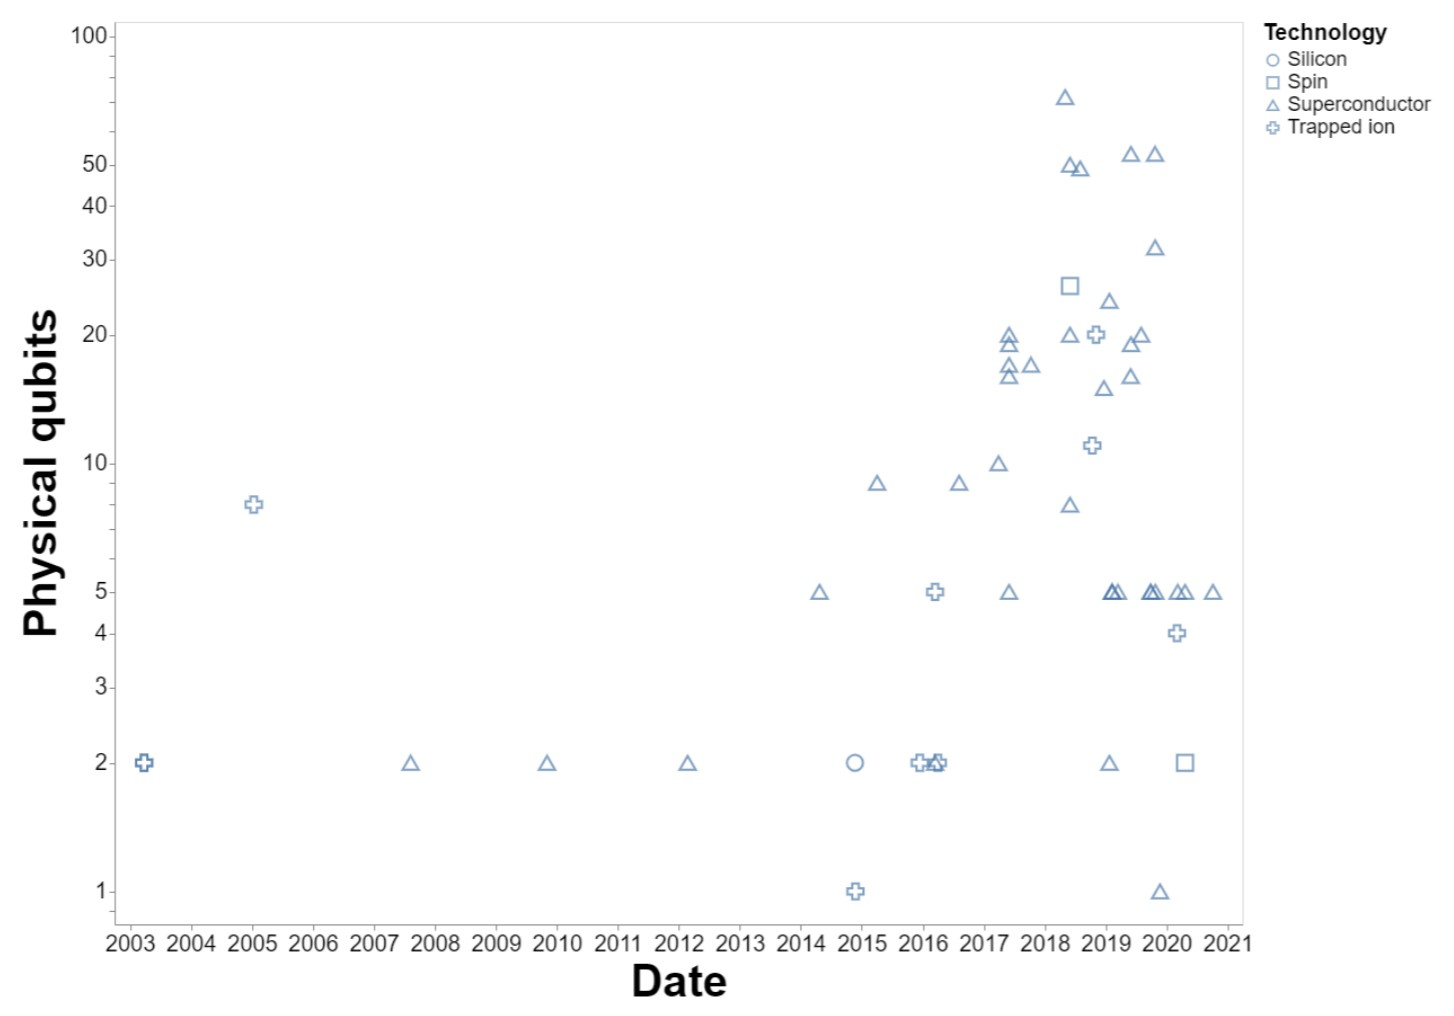
\includegraphics[scale=0.4]{Physical qubit counts.jpg}
    \caption{Physical qubit counts for 52 systems from 2003-2020. Figure from Sevilla and Riedel \cite{sevilla2020forecasting}}
    \label{fig:my_label}
\end{figure}

From the industrial side, IBM is the most forthright with their full timelines, but IonQ also provide a timeline for so called algorithmic qubit numbers, with both of these listed in the appendix. PsiQuantum are particularly ambitious, with their aim of over a million qubits on their first computer. 

\begin{figure}[htb]
    \centering
    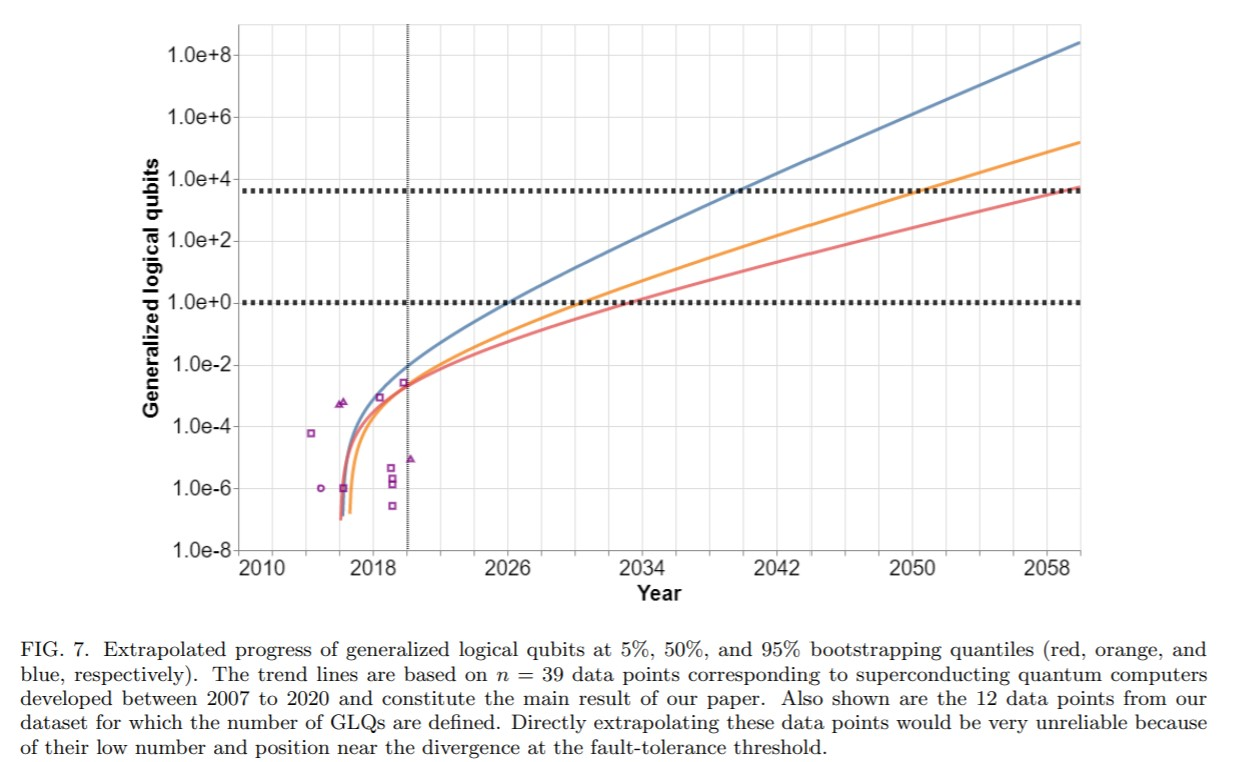
\includegraphics[scale=0.5]{Generalised logical qubit progress.jpg}
    \caption{Sevilla and Riedel's optimistic predictions for logical qubit progress}
    \label{fig:my_label}
\end{figure}




\clearpage
\part{A Mathematical Formulation}
This is where the maths is going to become a little heavier. We'll recap the basics from a firmer footing, and also touch on some places in the previous part that I'd like to have more maths in. Then we'll move on to some quantum machine learning, discuss current viable techniques and techniques that may be viable in the future. 
\section{Revisiting the Basics}
We specified, in Part I, that the most basic element of the quantum computer was the qubit. Typically, we represent these in \textbf{bra-ket notation}, with the simplest qubits being written as
\[
\ket{0}, \quad \ket{1}.
\]
We call the notation for these states, kets. We extend these to linear combinations like
\[
 \frac{1}{\sqrt{2}} (\ket{0} + \ket{1}).
\]
These are generalised to \textbf{superpositions}
\[
\ket{\psi} = \alpha \ket{0} + \beta \ket{1}, | \alpha |^2 + | \beta |^2 =1; \quad \alpha, \beta \in \mathbb{C}
\]
i.e. where $\alpha, \beta$ are complex numbers that live on the surface of a sphere with radius 1. We refer to this sphere as the Bloch sphere, and it represents all possible states for a qubit.

(Bloch sphere image goes here)

Classical bits are easily measured, since a 0 is a 0 and a 1 is a 1, but our qubits are linear combinations of these 0's and 1's, so how do we measure qubits like the ones above? Measurements of a state (of a qubit) give a single outcome, with probability determined by the state, and the choice of measurement we make. In general, we will measure in the \textbf{computational basis}, where the states are represented by 0's and 1's. In the above example, we obtain 0 with probability $|\alpha|^2$ and 1 with probability $| \beta|^2$. From this, we can see that our simple states $\ket{0}$  is measured to be 0 with certainty every single time. This is exactly as we would hope for, since it is essentially a classical state. In our other example, we can see that we obtain 0 or 1 with probability $1/2$. 

To generalise measurements, we need to consider bras. When given a ket, we can transform it into a bra via the Hermitian transpose, i.e.
\[
\bra{\psi} = (\ket{\psi})^\dagger = (\alpha \ket{0} + \beta \ket{1})^\dagger = \alpha^\ast \bra{0} + \beta^\ast \bra{1}.
\]
Now, given a state $\ket{\psi}$, we can compute the probability of obtaining a 0 as
\[
p(0) = \bra{\psi} P_0 \ket{\psi} = \braket{\psi | 0} \braket{0 | \psi} = |\braket{0 | \psi}|^2 = | \alpha | ^2.
\]
With the products $\braket{i | j} = \delta_{ij}$.

Measuring the states causes the state to collapse into the measured state, so if measure a state as a 0 and repeatedly measure the state, we will always measure a 0.

Bra-ket notation is standard for quantum computing, but we can also consider this from a vectorial representation.

\[
\ket{0} = \begin{pmatrix} 1 \\ 0\end{pmatrix}, \quad \ket{1} = \begin{pmatrix} 0 \\ 1 \end{pmatrix}.
\]
So, you can instead write state vectors as 
\[
\ket{\psi} = \begin{pmatrix} \alpha \\ \beta \end{pmatrix}, \quad |\alpha |^2 + | \beta|^2 = 1 ; \quad \alpha, \beta \in \mathbb{C}.
\]
Mimicking classical bit strings, we can also combine the qubits to form higher dimensional systems e.g.

\[
\ket{\psi} = \frac{1}{\sqrt{2}} (\ket{0} + \ket{1})  \otimes \frac{1}{\sqrt{2}} (\ket{0} + \ket{1}) = \frac{1}{2} (\ket{00} + \ket{01} + \ket{10} + \ket{11}).
\]
Measuring these product states is just an extension of measuring the single qubits and in the computational basis, we can read off probabilities by squaring the amplitude of the state(s) we're interested in. 

In higher dimensions, we can also introduce \textbf{entanglement}. One such example of an entangled state is the so-called EPR pair
\[
\ket{\Phi^+} = \frac{1}{\sqrt{2}}( \ket{00} + \ket{11}).
\]
It's clear that if we measure this state in the first qubit and obtain e.g a 0, then measuring the second qubit will also obtain a 0 with certainty. More generally, an $n$ dimensional entangled state is one that can't be written as a product of $n$ states. It's fairly simple to prove the above state is entangled by contradiction:
\[
\ket{\Phi^+} = (a \ket{0} + b \ket{1}) ( c \ket{0} + d \ket{1}) = ac \ket{00} + ad \ket{01} + bc \ket{10} + bd \ket{11}.
\]
Now, the form of $\ket{\Phi^+}$ gives us that $ad = bc = 0$, and that $ac = bd = \frac{1}{\sqrt{2}}$. But the first condition gives us that at least two of $a,b,c,d$ must be $0$, thus contradicting the second. So we conclude that $\ket{\Phi^+}$ is entangled. 



\section{Quantum Volume}
Note that this section is very maths heavy, a brief summary of calculating quantum volume is that the quantum computer attempts to solve a specific problem with a high probability. Success at certain depths of quantum circuits or qubit numbers are logged, and this number is transformed into a quantum volume. 

To introduce quantum volume, we first need to introduce another error source and another property of quantum computers. Connectivity is, simply, the number of other qubits a qubit is connected to and hence can interact with via 2-qubit gates. Crosstalk is errors caused by unintended local interactions of qubits, either stationary or caused by gates. 

Another metric for comparing quantum computers is the idea of \textbf{quantum volume}, introduced by IBM in Cross et al. \cite{Cross_2019}. This is another measure that takes into account the number of qubits available, gate errors, crosstalk and connectivity. However, this is a metric calculated by running a specific algorithm on the quantum computer, rather than being calculated directly from known qubits and error rates. Quantum volume is measured in powers of 2. 

\begin{table}[htb]
    \centering
    \begin{tabular}{ccc}
         Designation & Qubits & Quantum Volume  \\
        \hline
        Dublin & 27 & 64 \\
        Kolkata & 27 & 128 \\
        Manhattan & 65 & 32 
    \end{tabular}
    \caption{Quantum Volume for IBM Computers}
    \label{tab:quantum_volume_ibm}
\end{table}

From the above table, it's clear that increasing the number of qubits won't necessarily increase the quantum volume. Certainly, there comes a point when the quantum volume is more important than the number of qubits available.

Quantum volume is calculated based on how well the computer can solve the \textbf{heavy output generation} problem for random model circuits. (The gates picked for the circuit are from the Haar measure over SU(4)). 

The heavy set is given by
\[
H_U = \{ x \in \{0, 1\}^m : p_U (x) > p_{\text{med}} \}, \quad p_U = | \bra{x} U \ket{0} |^2,
\]
and $p_{\text{med}}$ is the median of these probabilities. The heavy output problem, then, is to generate a set of strings such that more than $2/3$ of them are heavy. In practice, for a given model circuit $U$, the computer implements an approximation $U'$ such that the average fidelity
\[
F_{\text{avg}} (U, U') = \frac{|\text{Tr} (U^\dagger U')|^2 / 2^m + 1}{2^m + 1}
\]
is close to 1. $h_U$ is then our probability that an output string from $U'$ is in the heavy set of $U$. We integrate $h_U$ over all appropriate model circuits i.e over the Haar measure on SU(4) to obtain $h_d$.

We define the achievable model circuit depth $d(m)$ to be the largest $d$ such that we are confident $h_d > 2/3$. Finally, we can define the quantum volume as
\[
\log_2 V_Q = \text{argmax}_m \min (m, d(m)) 
\]
i.e. the largest square shaped circuit we can implement. 

It's important that we are using random circuits rather than bench-marking using very specific circuits for certain quantum algorithms, since this imitates the circuits needed to load classical data on a quantum computer. 


\section{Quantum Embeddings}
Quantum embedding is the process of converting classical data points into quantum states, i.e. a feature map. There are several methods we can use to achieve this, each one giving rise to a corresponding kernel. Note that these embeddings (and more) are all available via the Pennylane Python library.

\begin{itemize}
    \item \textbf{Basis Encoding} - If we are given binary inputs, we can encode strings directly into state vectors e.g.
    \[
    010100 \to \ket{010100}.
    \]
    The kernel is given by the Kronecker delta $\delta_{ij}$. This is useful for binary optimisation problems like job ordering. 
    \item \textbf{Amplitude Encoding} - We can convert vectors straight to states by normalising them, e.g. 
    \[
    \mathbf{x} = (x_0 , \ldots, x_{N_1} )^T \in \mathbb{R}^N, \quad \mathbf{x} \to \ket{\psi_{\mathbf{x}}} = \frac{1}{\| \mathbf{x}\|_2} \sum_{i = 0}^{N-1} x_i \ket{i}
    \]
    With a (normalised) linear kernel. We can extend this to a product state with $d$ copies of the state to obtain the polynomial kernel, with power $d$.
    \item \textbf{Product Encoding} - Instead of normalising the vector, we can rescale the values into the intervals $[-\pi, \pi]$ and encode the features into the amplitudes of the qubits
    \[
    \mathbf{x} \to \ket{\psi_{\mathbf{x}}} = \prod_{i=0}^{N-1} (\cos (x_i) \ket{0} + \sin (x_i) \ket{1}).
    \]
    With the kernel, the cosine kernel. 
\end{itemize}

Following Lloyd et al. \cite{lloyd2020quantum} we can extend this to 
\[
\mathbf{x} \to \ket{\mathbf{x}} = \Phi(x, \theta) \ket{0 \ldots 0}.
\]
Where $\theta$ is a vector of physical parameters used as free variables for optimisation. In a technique called  propose that adaptive training should occur on the embedding, in order to create maximum separation in the feature space. This is an example of a variational quantum algorithm - we'll see more of this later.

\begin{figure}[htb]
    \centering
    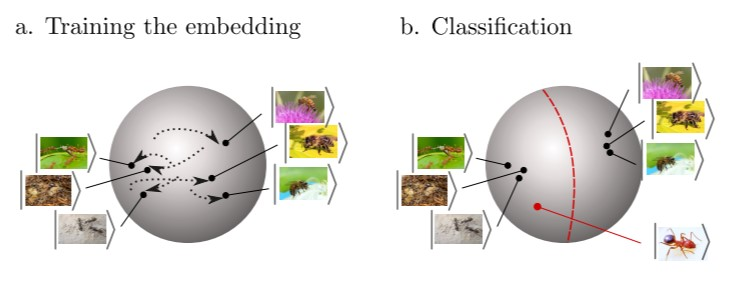
\includegraphics{Quantum Metric Learning.jpg}
    \caption{Quantum Metric Learning illustration from Lloyd et al. \cite{lloyd2020quantum}}
    \label{fig:quantum_metric_learning}
\end{figure}


\section{qRAM}
Quantum Random Access Memory (qRAM), is the quantum version of RAM. One such architecture for this comes from Giovannetti et al. \cite{Giovannetti_2008} and is dubbed bucket-brigade. The idea is to create a circuit that, if given addresses $\psi_i$ on $N$ memory cells, we can retrieve the stored memory in efficient ($O(\log N)$) time. For typical classical and quantum RAM stored in a $d$-dimensional lattice, you need $O(N^{\frac{1}{d}})$ switches. Given that this method has time requiring exponential speedup, we see that retrieving states from this would limit the data loading parts of the algorithms.

\[
\sum_i \psi_i \ket{i} \to \sum_i \psi_i \ket{i} \ket{M_i}
\]

Let's first consider the classical implementation. This method requires the uses of a trit taking one of three values, wait, left and right. Any trit in the wait states will change state when it receives one bit. A value of 0 will change the state to left and 1 to right then, any incoming bits are redirected accordingly. To retrieve information, we begin the protocol will all trits in the wait state. We send the address, a bit string, through the lattice and create a path to the desired memory cell. A bus signal is then sent through the lattice, which follows the path carved out and retrieves the information from the cell. When travelling through the lattice, it resets all the trits to the wait states, thus returning the system to its initial state. 

\tikzset{every picture/.style={line width=0.75pt}} %set default line width to 0.75pt        

\begin{figure}[htb]
    \centering
    \begin{tikzpicture}[x=0.75pt,y=0.75pt,yscale=-1,xscale=1]
%uncomment if require: \path (0,323); %set diagram left start at 0, and has height of 323

%Shape: Rectangle [id:dp06324507221689823] 
\draw   (200,90) -- (260,90) -- (260,130) -- (200,130) -- cycle ;

%Shape: Rectangle [id:dp9904458770833908] 
\draw   (280,30) -- (340,30) -- (340,70) -- (280,70) -- cycle ;

%Shape: Rectangle [id:dp1498155222936699] 
\draw   (400,160) -- (460,160) -- (460,200) -- (400,200) -- cycle ;

%Shape: Rectangle [id:dp32386546467729516] 
\draw   (240,160) -- (300,160) -- (300,200) -- (240,200) -- cycle ;

%Shape: Rectangle [id:dp5339748375708644] 
\draw   (160,160) -- (220,160) -- (220,200) -- (160,200) -- cycle ;

%Shape: Rectangle [id:dp9913931908830227] 
\draw   (320,160) -- (380,160) -- (380,200) -- (320,200) -- cycle ;

%Shape: Rectangle [id:dp9560489881446825] 
\draw   (360,90) -- (420,90) -- (420,130) -- (360,130) -- cycle ;

%Rounded Rect [id:dp024913878313268745] 
\draw   (160,234) .. controls (160,231.79) and (161.79,230) .. (164,230) -- (176,230) .. controls (178.21,230) and (180,231.79) .. (180,234) -- (180,266) .. controls (180,268.21) and (178.21,270) .. (176,270) -- (164,270) .. controls (161.79,270) and (160,268.21) .. (160,266) -- cycle ;
%Rounded Rect [id:dp5941558202230157] 
\draw   (200,234) .. controls (200,231.79) and (201.79,230) .. (204,230) -- (216,230) .. controls (218.21,230) and (220,231.79) .. (220,234) -- (220,266) .. controls (220,268.21) and (218.21,270) .. (216,270) -- (204,270) .. controls (201.79,270) and (200,268.21) .. (200,266) -- cycle ;
%Rounded Rect [id:dp759094812942045] 
\draw   (240,234) .. controls (240,231.79) and (241.79,230) .. (244,230) -- (256,230) .. controls (258.21,230) and (260,231.79) .. (260,234) -- (260,266) .. controls (260,268.21) and (258.21,270) .. (256,270) -- (244,270) .. controls (241.79,270) and (240,268.21) .. (240,266) -- cycle ;
%Rounded Rect [id:dp16852035026538603] 
\draw   (280,234) .. controls (280,231.79) and (281.79,230) .. (284,230) -- (296,230) .. controls (298.21,230) and (300,231.79) .. (300,234) -- (300,266) .. controls (300,268.21) and (298.21,270) .. (296,270) -- (284,270) .. controls (281.79,270) and (280,268.21) .. (280,266) -- cycle ;
%Rounded Rect [id:dp5358481912780362] 
\draw   (320,234) .. controls (320,231.79) and (321.79,230) .. (324,230) -- (336,230) .. controls (338.21,230) and (340,231.79) .. (340,234) -- (340,266) .. controls (340,268.21) and (338.21,270) .. (336,270) -- (324,270) .. controls (321.79,270) and (320,268.21) .. (320,266) -- cycle ;
%Rounded Rect [id:dp3115101069190793] 
\draw   (360,234) .. controls (360,231.79) and (361.79,230) .. (364,230) -- (376,230) .. controls (378.21,230) and (380,231.79) .. (380,234) -- (380,266) .. controls (380,268.21) and (378.21,270) .. (376,270) -- (364,270) .. controls (361.79,270) and (360,268.21) .. (360,266) -- cycle ;
%Rounded Rect [id:dp05080113507368633] 
\draw   (400,234) .. controls (400,231.79) and (401.79,230) .. (404,230) -- (416,230) .. controls (418.21,230) and (420,231.79) .. (420,234) -- (420,266) .. controls (420,268.21) and (418.21,270) .. (416,270) -- (404,270) .. controls (401.79,270) and (400,268.21) .. (400,266) -- cycle ;
%Rounded Rect [id:dp21629845307422713] 
\draw   (440,234) .. controls (440,231.79) and (441.79,230) .. (444,230) -- (456,230) .. controls (458.21,230) and (460,231.79) .. (460,234) -- (460,266) .. controls (460,268.21) and (458.21,270) .. (456,270) -- (444,270) .. controls (441.79,270) and (440,268.21) .. (440,266) -- cycle ;
%Straight Lines [id:da9309903889218856] 
\draw    (310,70) -- (230,90) ;
%Straight Lines [id:da31341899039231724] 
\draw    (230,130) -- (190,160) ;
%Straight Lines [id:da260660362796477] 
\draw [color={rgb, 255:red, 208; green, 2; blue, 27 }  ,draw opacity=1 ]   (310,70) -- (390,90) ;
%Straight Lines [id:da5797342852502194] 
\draw    (230,130) -- (270,160) ;
%Straight Lines [id:da020677020049298278] 
\draw    (190,200) -- (170,230) ;
%Straight Lines [id:da663030675713139] 
\draw    (210,230) -- (190,200) ;
%Straight Lines [id:da41885221770083847] 
\draw    (270,200) -- (250,230) ;
%Straight Lines [id:da9194785373230423] 
\draw    (270,200) -- (290,230) ;
%Straight Lines [id:da03024275828416645] 
\draw    (390,130) -- (350,160) ;
%Straight Lines [id:da4396347581665594] 
\draw [color={rgb, 255:red, 208; green, 2; blue, 27 }  ,draw opacity=1 ]   (390,130) -- (430,160) ;
%Straight Lines [id:da6990591050773454] 
\draw [color={rgb, 255:red, 208; green, 2; blue, 27 }  ,draw opacity=1 ]   (430,200) -- (410,230) ;
%Straight Lines [id:da039909187532149115] 
\draw    (350,200) -- (330,230) ;
%Straight Lines [id:da9394370516012303] 
\draw    (350,200) -- (370,230) ;
%Straight Lines [id:da8756852263957238] 
\draw    (430,200) -- (450,230) ;

% Text Node
\draw (291,42) node [anchor=north west][inner sep=0.75pt]   [align=left] {Right};
% Text Node
\draw (214,102) node [anchor=north west][inner sep=0.75pt]   [align=left] {Wait};
% Text Node
\draw (254,172) node [anchor=north west][inner sep=0.75pt]   [align=left] {Wait};
% Text Node
\draw (174,172) node [anchor=north west][inner sep=0.75pt]   [align=left] {Wait};
% Text Node
\draw (334,172) node [anchor=north west][inner sep=0.75pt]   [align=left] {Wait};
% Text Node
\draw (371,102) node [anchor=north west][inner sep=0.75pt]   [align=left] {Right};
% Text Node
\draw (417,172) node [anchor=north west][inner sep=0.75pt]   [align=left] {Left};


\end{tikzpicture}
    \caption{Bucket Brigade architecture for qRAM with 8 memory cells}
    \label{fig:bucket_brigade}
\end{figure}

With the quantum system, we replace the trits with qutrits (or qudits with $d=3$) and similarly promote these states to $\ket{\text{wait}}, \ket{\text{left}} , \ket{\text{right}}$. At each of the nodes of the graph, if we encounter a $\ket{\text{wait}} $ we now apply a unitary transformation $U$ 

\[
U \ket{0} \ket{\text{wait}} = \ket{f} \ket{\text{left}} , \quad U \ket{1} \ket{\text{wait}} = \ket{f} \ket{\text{right}}.
\]
If we encounter either $\ket{\text{left}} $ or $\ket{\text{right}}$, we continue to route the address down this path. If we send a superposition of states into the lattice, by linearity we then obtain a corresponding superposition of paths through the lattice, allowing us to access the memory cells in superposition with our quantum bus. When returning, the bus applies $U^\dagger $ at each node, so that
\[
  U^\dagger \ket{f} \ket{\text{left}} =  \ket{0} \ket{\text{wait}} , \quad U^\dagger \ket{f} \ket{\text{right}} = \ket{1} \ket{\text{wait}} 
\]
and the lattice is returned to its original state. Taking $N=8$, we could for example send the code

\[
\ket{\psi} = \frac{1}{\sqrt{3}} ( \ket{101} + \ket{011} + \ket{000}),
\]
which would return an equal superposition of the states in 0th, 3rd and 5th memory cells. 

However, progress with qRAM has been slow. Consider that in order to use qRAM we still require $O(N)$ qutrits, so even storing $8$ states requires a minimum of $12$ qudits to retrieve a basic quantum state. (In fact precisely $N$ qutrits, $\log N $ qubits to access the memory and an ancilla the size of the state being accessed). Thus, to effectively use qRAM for machine learning this implementation would likely need thousands of qubits. An alternative approach by Jiang et al. \cite{Jiang} has shown a proof-of-concept realisation of 105 qubits, stored in 210 memory cells. 


\section{Quantum Machine Learning}
There are a number of machine learning algorithms in classical computing that have quantum counterparts. The first stage of most of these algorithms is embedding. Typically, this is achieved either by amplitude encoding or loading data from qRAM. 

Far more quantum algorithms exist, than we can conceivably cover in this report, so we'll focus on a key few. You can find many of these at \verb|https://quantumalgorithmzoo.org/|

\begin{itemize}
    \item Quantum Principal Component Analysis \cite{Lloyd_2014}
    \item $k$-means Clustering \cite{lloyd2013quantum}
    \item Support Vector Machines \cite{Rebentrost_2014}
    \item Linear Regression \cite{Schuld_2016}
\end{itemize}

Of these, on NISQ computers, the support vector machines are the only algorithms with current practical use. Quantum PCA and k-means clustering rely on qRAM or efficient state loading plus efficient Hamiltonian simulation \cite{Lloyd1073}.

As mentioned above, many classical machine learning algorithms have quantum counterparts, but the same is true of quantum algorithms with classical counterparts. Quantum inspired optimisation (QIO) algorithms take quantum algorithms and apply similar techniques to purely classical computations. Quantum principal component analysis has a corresponding classical algorithm also in polynomial $\log N$ time \cite{tang2019quantuminspired}, although requires efficient implementation of a similar starting state to 

\section{Quantum PCA}
The main result of LLoyd et al. \cite{Lloyd_2014} is the ability to construct the exponentiation of a density matrix for low rank matrices, i.e. given $\rho$ we can construct $e^{- i \rho t}$. Quantum PCA follows from our ability to apply the quantum phase estimation algorithm using this matrix \cite{10.5555/1972505}. 

Quantum phase estimation: Given unitary operator in $d$ dimensions and eigenstate $\ket{v_{\phi}} : U\ket{v_{\phi}} = e^{ 2 \pi i \phi} \ket{v_{\phi}}$. We want to estimate the phase $\phi$ for $0 < \phi < 1$ to $n$ binary bits of precision,
 \[
 \phi \approx 0.i_1i_2\ldots i_n = \frac{i}{2} + \frac{i_2}{4} + \cdots + \frac{i_n}{2^{n}}, \quad i_j \in \{0,1\} 
 .\] 
 We'll need controlled $U^{k}$ for integers $k$.
  \[
      C-U^{k} \ket{0}\ket{\psi} = \ket{0}{\ket\psi}, \quad C-U^{k}\ket{1}\ket{\psi} = \ket{1}(U^{k}\ket{\psi})
 .\] 
We'll actually want "generalised controlled  $U^{k}$ " 
\[
    \ket{x} \ket{\psi} \to \ket{x} U^{x} \ket{\psi}, \quad x\in  \mathbb{Z}_{2^{n}}
.\]

\begin{figure}[htb]
    \centering
        \begin{quantikz}
&	\lstick{$\ket{x_{n-1}}$} & \qw & \qw &  \qw & \cdots & \ctrl{4} \\
&	\lstick{\vdots} & \vdots & \vdots &  &\vdots & \vdots \\
&	\lstick{$\ket{x_1}$} &\qw & \ctrl{2} & \qw & \cdots & \qw \\
&	\lstick{$\ket{x_0}$} & \ctrl{1} & \qw  & \qw & \cdots & \qw  \\
& \lstick{$\ket{v}$} & \gate{U^{2^0}} & \gate{U^{2^1}} & \qw &\cdots & \gate{U^{2^{n-1}}} 
	\end{quantikz}
    \caption{Circuit to implement $\ket{x} \ket{v} \to \ket{x} U^x \ket{v} $, for $x = x_{n - 1} \cdots x_1 x_0 = x_0 + 2 x_1 + 2^2 x_2 + \cdots 2^{n-1} x_{n-1}, x \in \mathbb{Z}_{2^n}$ }
    \label{fig:my_label}
\end{figure}

Note: if input $\ket{\psi}  = \ket{v_{\phi}}$, then we get $e^{ 2 \pi i \phi x} \ket{x}\ket{v_{\phi}}$. \\


The general algorithm is as follows:  superpose over all $x = 0, 1, 2, \ldots, 2^{n - 1}$ and use $\ket{\psi } = \ket{v_{\phi}}$
Finally, apply $QFT_{2^{n}}$ to the resulting state and measure to see $y_0, y_1, \ldots, y_{n -1}$ on lines $0,1, \ldots, n-1$ then output the number
\[
0.y_0y_1\ldots y_{n - 1} = \frac{y_0}{2} + \frac{y_1}{4} + \cdots + \frac{y_{n - 1}}{2^{n}}
,\]
as an estimate of $\phi$. That's the phase estimation algorithm (for given $U$ and $\ket{v_{\phi}}$. \\
Suppose $\phi$ actually only had $n$ binary digits i.e. $ \phi = 0.z_0 z_1 \ldots z_{n - 1}$ for some $z_0, \ldots, z_{n-1}$ then
\[
\phi = \frac{z_0z_1\cdots z_{n-1}}{2^{n}} = \frac{z}{2^{n}}
,\]
for $z$ an $n$ bit integer in $\mathbb{Z}_{2^{n}}$ and 
\[
    \ket{A} = \frac{1}{\sqrt{2^{n}}} \sum_{x} e^{ 2 \pi i \frac{x z}{2^{n}}} \ket{x}  
\]
is $QFT$ of $\ket{z}$. So  $QFT^{-1} \ket{A} = \ket{z}$ and we get $\phi$ exactly and with certainty. \\
Note: in this case, the PE algorithm up to and not including the final measurement is a unitary operation $U_{PE}$ mapping
\[
    \ket{0} \ldots\ket{0} \ket{v_{\phi}} \to \ket{z_0} \ket{z_1} \ldots \ket{z_{n-1}} \ket{v_{\phi}}
.\] 
If $\phi$ has more than $n$ bits
\[
\phi = 0.z_0z_1 \ldots z_{n - 1} ; z_{n } z_{n + 1}
,\]
then we have
\begin{thm}[Phase Estimation]
If measurements in the above algorithm give $y_0, y_1, \ldots, y_{n - 1}$ so output is $\theta = 0.y_0 y_1 \ldots y_{n-1} $ then 
\begin{itemize}
    \item $P( \theta \text{ is closest } n \text{ binary digit approx to } \phi ) \ge \frac{4}{\pi ^2} \approx 0.4$ 
    \item $P(\mid \theta - \phi \mid  \ge \varepsilon)$ is at most $O\left( \frac{1}{2^{n} \varepsilon} \right) $.
\end{itemize}
\end{thm}

If we take a general state $\ket{\psi}$ instead, and use $U = e^{- i \rho }$ for our density matrix $\rho$, then we can take 

\[
\ket{\psi} \ket{0} \to \sum_i a_i \ket{v_{\phi_i}} \ket{\tilde{\lambda}_i},
\]
where $\ket{v_{\phi_i}}$ are the eigenvectors of $\rho$ and $\tilde{\lambda}_i$ are the corresponding eigenvalue estimates. LLoyd et al \cite{Lloyd_2014} suggest using $\rho$ as the initial state, so the algorithm gives the final state
\[
\sum_i \lambda_i \ket{v_{\phi_i}}  \bra{v_{\phi_i}} \otimes \ket{\tilde{\lambda}_i} \bra{\tilde{\lambda}_i}.
\]
Sampling from this state allows us to obtain information about the eigenvalues and eigenstates of the density matrix.

\section{Variational Quantum Algorithms}
Variational quantum algorithms (VQAs) are a growing class of machine learning options. A detailed review of the field is given in \cite{cerezo2020variational}. These are likely to be the most useful algorithms in the near term. 

VQAs tend to be most comparable to classical neural networks, and can be thought of as a class of hybrid    quantum-classical algorithms. 

We begin by casting the problem we wish to solve as the solution to an optimisation
\[
\ket{\Psi^\ast} = \text{argmin}_{\ket{\Psi}} \bra{\Psi} H \ket{\Psi},
\]
such that the cost function $C(\ket{\psi}) = \bra{\Psi} H \ket{\Psi}$ is a faithful representation of the problem. We construct an entangling quantum circuit of low depth - this is due to constraints on NISQ computers and $log_2$ of the quantum volume should give the maximum circuit depth you can use. It's also important that the circuit is entangling, else we gain no quantum advantage and this process is equivalent to a classical optimisation task.

\begin{figure}[htb]
    \centering
    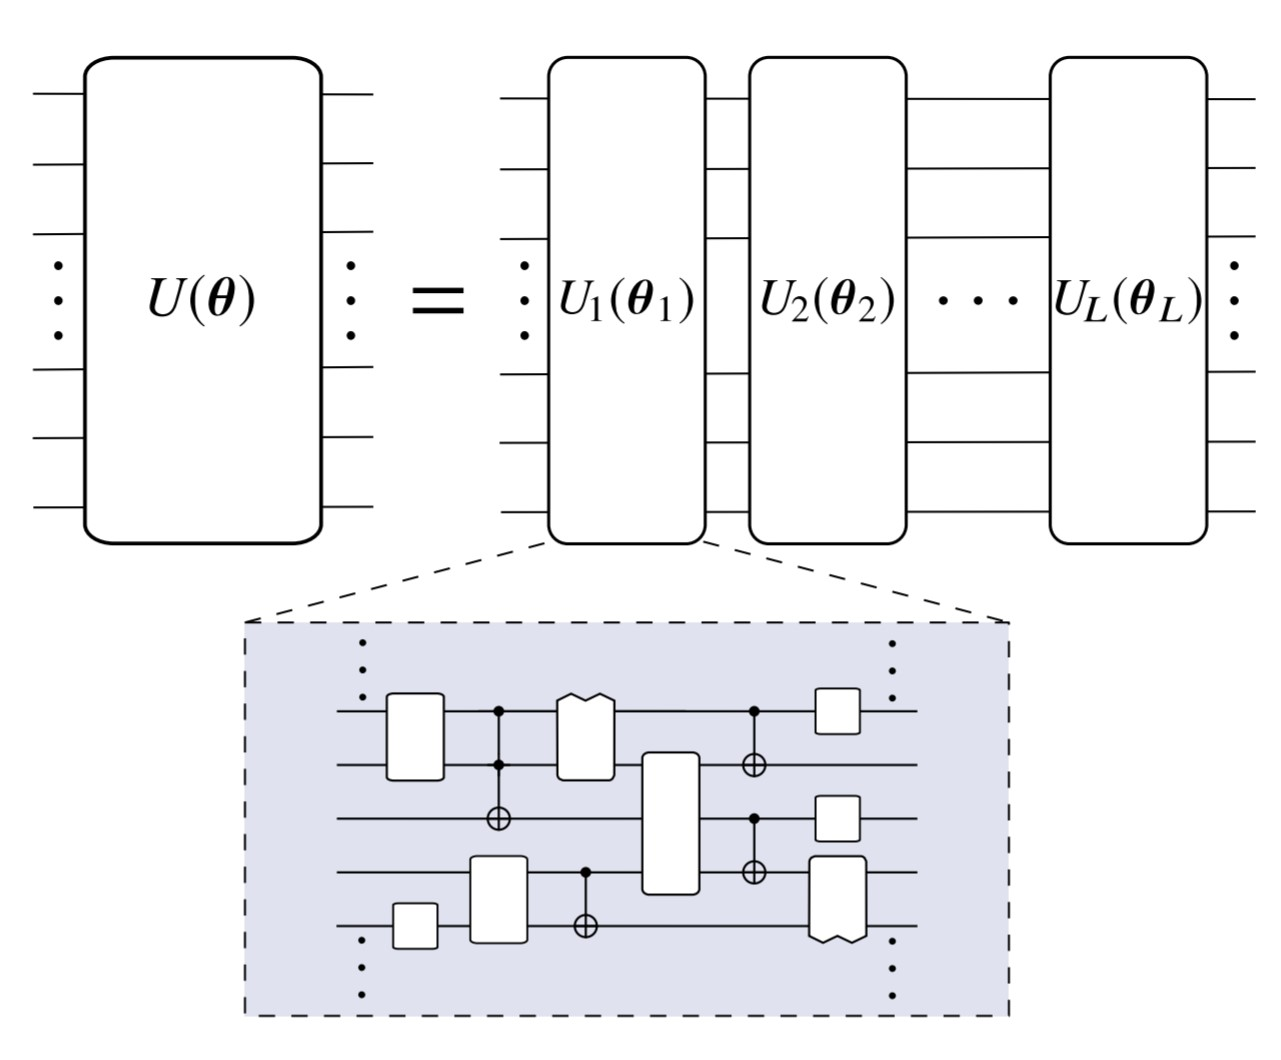
\includegraphics[scale=0.3]{VQA.jpg}
    \caption{Parameterised Quantum Circuit \cite{cerezo2020variational}. }
    \label{fig:my_label}
\end{figure}

We then train an optimiser on a set of data using either parameter-shift \cite{crooks2019gradients} or backpropagation \cite{watabe2019quantum}.

%\section{Quantum Annealing}
%In the space of optimisation solutions, quantum also offers an annealing solution. Classical annealing is based on the idea of slowly cooling a system down


\section{Existing Examples}
Pennylane has a number of tutorials for quantum machine learning examples. This mostly follows \\ \verb|https://pennylane.ai/qml/demos/tutorial_ensemble_multi_qpu.html|, an ensemble method, classifying data from the Iris dataset. Two classifiers have been pre-trained on quantum circuits, so this is verification of parameters rather than hyper-parameter tuning. Two computations are run in parallel on quantum computers, and three qubits are measured in the computational basis. For every measurement taking value 0 we, assign it 1, and for every measurement taking value 1, we assign it -1. We then average over all such measurements,  and rescale to obtain classification probabilities. For a given piece of data, we assign the class that has the highest probability from either of the two circuits, i.e. the circuit that is most certain, picks the class. 

Both circuits use product encoding, with a rotation around the x-axis of the Bloch sphere.

\[
R_x(\phi) = e^{ - i \phi \sigma_x / 2} = \begin{pmatrix} \cos ( \phi / 2) & - i \sin (\phi / 2) \\ - i \sin( \phi / 2) & \cos(\phi / 2)
\end{pmatrix},
\]
as well as general rotation gates controlled by a set of 16 training parameters 
\[
\theta_{ij}^{(k)} \in [- \pi, \pi)^3 ; \quad  i,k \in \{0,1\}, \quad j \in \{0,1,2,3\}.
\]
General rotations are given by
\[
R(\phi, \theta, \omega) = R_z(\omega)R_y(\theta)R_z(\phi) = \begin{pmatrix} e^{-i ( \phi + \omega) /2}\cos ( \theta / 2) & - e^{-i ( \phi - \omega) /2} \sin (\theta / 2) \\ e^{-i ( \phi - \omega) /2} \sin( \theta / 2) &  e^{i ( \phi + \omega) /2}\cos(\theta / 2)
\end{pmatrix}
\]



\begin{figure}[htb]
    \centering
        \begin{quantikz}
&	\lstick{$\ket{0}$} &\gate{R_x(x_0)} & \gate{R(\theta_{00}^{(0)})}  & \gate{Z}  & \qw & \gate{Z} &   \gate{R(\theta_{10}^{(0)})} & \meter{} \\
&	\lstick{$\ket{0}$} &\gate{R_x(x_1)} & \gate{R(\theta_{01}^{(0)})}  & \ctrl{-1}  & \ctrl{1} & \qw & \gate{R(\theta_{11}^{(0)})} &\meter{} \\
&	\lstick{$\ket{0}$} &\gate{R_x(x_0)} & \gate{R(\theta_{02}^{(0)})}  & \qw  & \gate{Z} & \qw & \gate{R(\theta_{12}^{(0)})} &\meter{} \\
&	\lstick{$\ket{0}$} &\gate{R_x(x_1)} & \gate{R(\theta_{03}^{(0)})}  & \qw  & \qw & \ctrl{-3} & \gate{R(\theta_{13}^{(0)})} &  \trash{\text{discard}} \\
	\end{quantikz}
    \caption{Device 0 Quantum Circuit}
    \label{fig:my_label}
\end{figure}
\begin{figure}[htb]
    \centering
        \begin{quantikz}
&	\lstick{$\ket{0}$} &\gate{R_x(x_0)} & \gate{R(\theta_{00}^{(1)})}  & \ctrl{1}  & \qw & \gate{Z} &   \gate{R(\theta_{10}^{(1)})} & \meter{} \\
&	\lstick{$\ket{0}$} &\gate{R_x(x_1)} & \gate{R(\theta_{01}^{(1)})}  & \gate{Z}  & \ctrl{1} & \ctrl{2} & \gate{R(\theta_{11}^{(1)})} &\meter{} \\
&	\lstick{$\ket{0}$} &\gate{R_x(x_0)} & \gate{R(\theta_{02}^{(1)})}  & \qw  & \gate{Z} & \qw & \gate{R(\theta_{12}^{(1)})} &\meter{} \\
&	\lstick{$\ket{0}$} &\gate{R_x(x_1)} & \gate{R(\theta_{03}^{(1)})}  & \qw  & \qw & \gate{Z} & \gate{R(\theta_{13}^{(1)})} &  \trash{\text{discard}} \\
	\end{quantikz}
    \caption{Device 1 Quantum Circuit}
    \label{fig:my_label}
\end{figure}
\begin{table}[htb]
    \centering
    \begin{tabular}{l|cc}
         & Training & Test  \\
         Ensemble & 0.8 & 0.64 \\ 
         QPU0 & 0.648 & 0.56\\
         QPU1 & 0.296 & 0.32
    \end{tabular}
    \caption{Accuracy of predictions using IBM's Manila and Santiago (5 qubit, 32 quantum volume) computers as devices 0 and 1 respectively. The training set had 125 pieces of data, and the test set 25.}
    \label{tab:my_label}
\end{table}


\clearpage
\part{Software Implementation}

\clearpage
\printbibliography
\clearpage

\appendix 
\section{Definitions and Acronyms}
\begin{itemize}
    \item FTQC - Fault Tolerant Quantum Computers
    \item NISQ - Noisy Intermediate Scale Quantum computers
    \item QAOA - Quantum Approximate Optimisation Algorithms
    \item QEC - Quantum Error Correction
    \item QIO - Quantum Inspired Optimisation
    \item qRAM - Quantum Random Access Memory
    \item VQA - Variational Quantum Algorithm
    \item VQE - Variational Quantum Eigensolver

\end{itemize}
\section{Industrial Timelines}
\begin{figure}[htb]
    \centering
    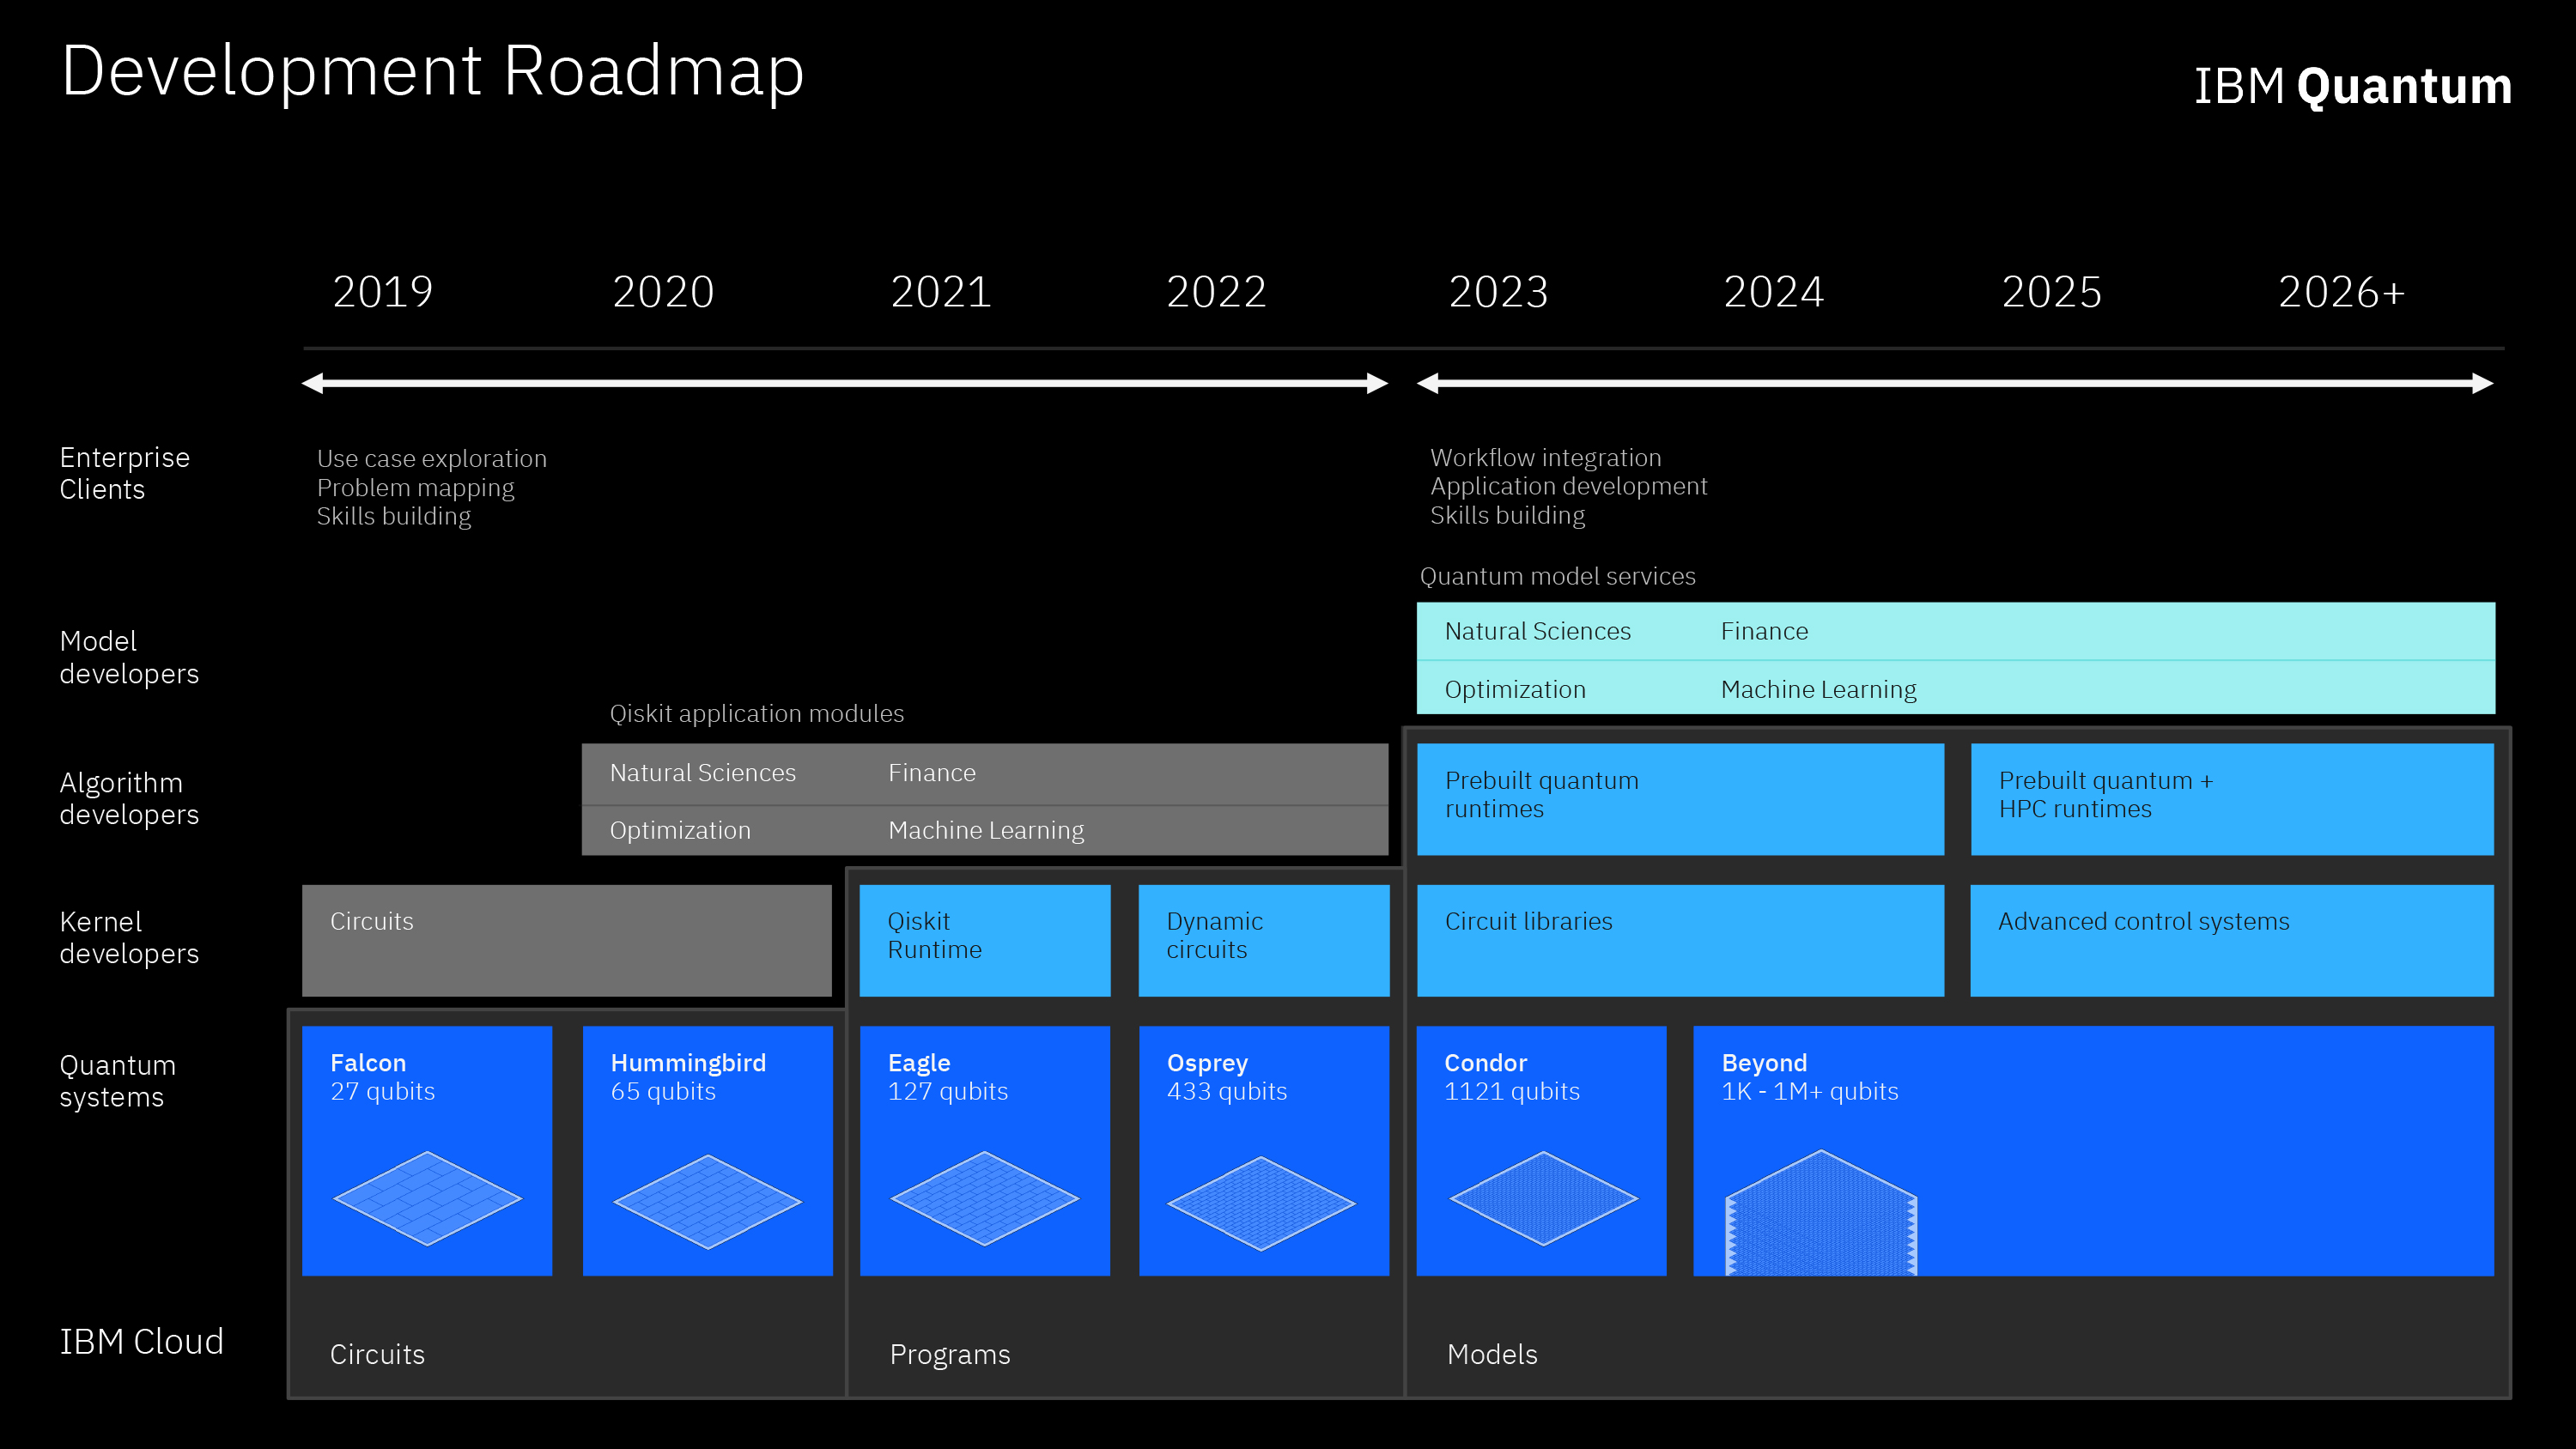
\includegraphics[scale=0.1]{50863431103_aa832db592_o.jpg}
    \caption{IBM timeline for Quantum Computing \cite{wehden_faro_gambetta_2021} }
    \label{fig:ibm_timeline}
\end{figure}

\begin{figure}[htb]
    \centering
    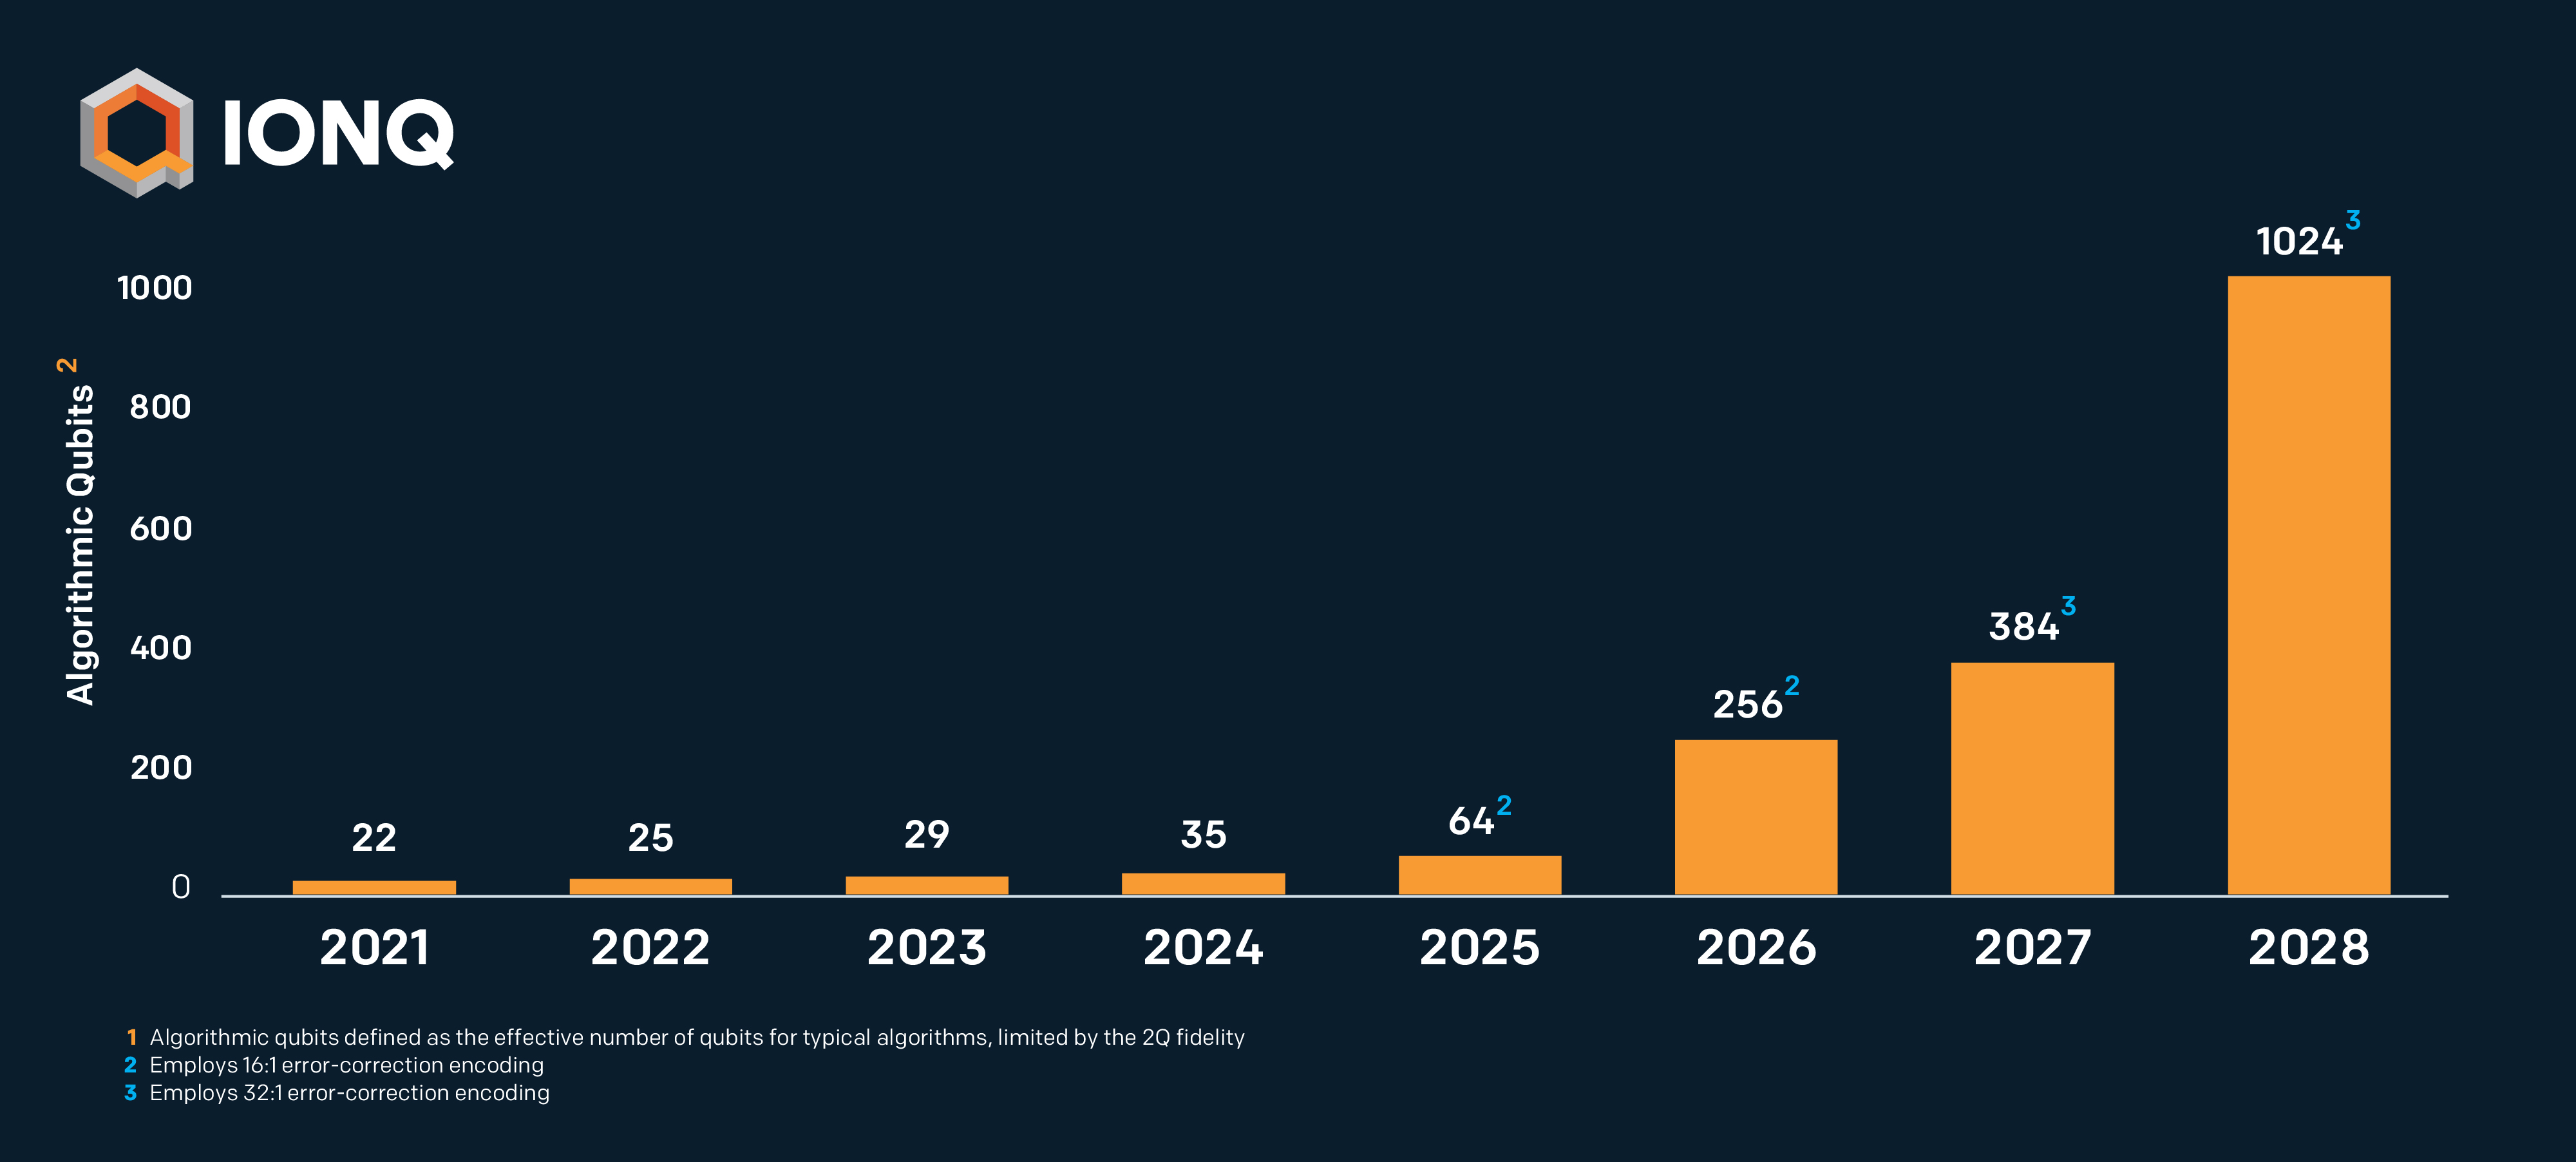
\includegraphics[scale=0.1]{IonQ-roadmap-20201208.jpg}
    \caption{IonQ Qubit Roadmap}
    \label{fig:IonW_timeline}
\end{figure}

\end{document}
